%% 
%% Copyright 2019-2021 Elsevier Ltd
%% 
%% This file is part of the 'CAS Bundle'.
%% --------------------------------------
%% 
%% It may be distributed under the conditions of the LaTeX Project Public
%% License, either version 1.2 of this license or (at your option) any
%% later version.  The latest version of this license is in
%%    http://www.latex-project.org/lppl.txt
%% and version 1.2 or later is part of all distributions of LaTeX
%% version 1999/12/01 or later.
%% 
%% The list of all files belonging to the 'CAS Bundle' is
%% given in the file `manifest.txt'.
%% 
%% Template article for cas-dc documentclass for 
%% double column output.

\documentclass[fleqn]{cas-sc}

\usepackage{lipsum}
\usepackage{tikz}
\usetikzlibrary{shapes, snakes, calc, positioning}
\usepackage{longtable}

% If the frontmatter runs over more than one page
% use the longmktitle option.

%\documentclass[a4paper,fleqn,longmktitle]{cas-dc}

%\usepackage[numbers]{natbib}
%\usepackage[authoryear]{natbib}
\usepackage[authoryear,longnamesfirst]{natbib}

%%%Author macros
\def\tsc#1{\csdef{#1}{\textsc{\lowercase{#1}}\xspace}}
\tsc{WGM}
\tsc{QE}
%%%

% Uncomment and use as if needed
%\newtheorem{theorem}{Theorem}
%\newtheorem{lemma}[theorem]{Lemma}
%\newdefinition{rmk}{Remark}
%\newproof{pf}{Proof}
%\newproof{pot}{Proof of Theorem \ref{thm}}

\begin{document}
\let\WriteBookmarks\relax
\def\floatpagepagefraction{1}
\def\textpagefraction{.001}

% Short title
\shorttitle{Ambulance Dispatch}    

% Short author
\shortauthors{Burkman, Chu, Jin, Abuhijleh, and Sun}  
%\shortauthors{First, Second, Third, Fourth}  

% Main title of the paper
\title [mode = title]{Recommendation System for Ambulance Dispatch based on Automated Crash Reports from Cell Phones}  

% Title footnote mark
% eg: \tnotemark[1]
%\tnotemark[<tnote number>] 
%\tnotemark[1] 

% Title footnote 1.
% eg: \tnotetext[1]{Title footnote text}
%\tnotetext[1]{Working Title} 

% First author
%
% Options: Use if required
% eg: \author[1,3]{Author Name}[type=editor,
%       style=chinese,
%       auid=000,
%       bioid=1,
%       prefix=Sir,
%       orcid=0000-0000-0000-0000,
%       facebook=<facebook id>,
%       twitter=<twitter id>,
%       linkedin=<linkedin id>,
%       gplus=<gplus id>]

%\author[<aff no>]{<author name>}[<options>]
\author[1,2]{J. Bradford Burkman}[]
%\author[1,2]{First Author}[]
% Footnote of the first author
\fnmark[1]
% Corresponding author indication
\cormark[1]
% Email id of the first author
\ead{bradburkman@gmail.com}
%\ead{FirstAuthor@gmail.com}
% URL of the first author
\ead[url]{http://www.github.com/bburkman}

% Credit authorship
% eg: \credit{Conceptualization of this study, Methodology, Software}
% Options: conceptualization; data curation; formal analysis; funding acquisition; investigation; methodology; project administration; resources; software; supervision; validation; visualization; writing – original draft; and writing – review and editing.
\credit{Conceptualization, Investigation, Writing - original draft, Visualization}

\author[1]{Chee-Hung Henry Chu}
\credit{Supervision, Methodology, Writing - review and editing}

\author[1]{Miao Jin}[]
%\author[1]{Second Author}[]
\credit{Supervision, Methodology}

\author[1,3]{Malek Abuhijleh}[]
%\author[1,3]{Third Author}[]
\credit{Data curation, Investigation, Methodology}

\author[3]{Xiaoduan Sun}[]
%\author[3]{Fourth Author}[]
\credit{Data curation, Writing - review and editing}





\affiliation[1]{organization={School of Computing and Informatics, University of Louisiana at Lafayette},
%\affiliation[1]{organization={School, University},
            addressline={301 E. Lewis St}, 
            city={Lafayette},
          citysep={}, % Uncomment if no comma needed between city and postcode
            state={LA},
            postcode={70503}, 
            country={USA}
            }

% Address/affiliation
\affiliation[2]{organization={Louisiana School for Math, Science, and the Arts},
%\affiliation[2]{organization={Other School},
            addressline={715 University Pkwy}, 
            city={Natchitoches},
          citysep={}, % Uncomment if no comma needed between city and postcode
            state={LA},
            postcode={71457}, 
            country={USA}
            }

\affiliation[3]{organization={Department of Civil Engineering, University of Louisiana at Lafayette},
%\affiliation[3]{organization={Other Department, University},
            addressline={131 Rex St}, 
            city={Lafayette},
          citysep={}, % Uncomment if no comma needed between city and postcode
            state={LA},
            postcode={70504}, 
            country={USA}
            }




% For a title note without a number/mark
%\nonumnote{}

% Here goes the abstract
\begin{abstract}
%%%%% Abstract
% I found an abstract in TRpC June 2022 with 365 words.
%Put abstract here.
%%%%% Abstract
% I found an abstract in TRpC June 2022 with 365 words.
Some new cell phones can automatically notify an emergency dispatcher if the phone detects the deceleration profile of a vehicular crash.  Most crash notifications come from an eyewitness who can say whether an ambulance is needed, but the automated notification from the cell phone cannot provide that information directly.  Should the dispatcher immediately send an ambulance before receiving an eyewitness report?  There are three options: Always, Wait, and Sometimes.  The ``Always'' option refers to sending an ambulance to every automatically reported crash, even though most of them will not be needed.  In the ``Wait'' option, the dispatcher sends police, but always waits for a call from an eyewitness (perhaps the police) before sending an ambulance.  In the ``Sometimes'' option, the dispatcher relies on a machine learning recommendation system to decide whether to immediately dispatch an ambulance, reserving the option to send one later based on an eyewitness report.

%This paper explores one option for building a machine learning (ML) model for making a recommendation in the ``Sometimes'' option.  The model gives the probability (based on the available information) that a crash requires an ambulance.  If the probability that an ambulance is needed is above some chosen threshold, the method will recommend dispatching an ambulance immediately; below that threshold, the dispatcher should wait to hear from an eyewitness. 


This paper explores one option for building a machine learning (ML) model for making a recommendation in the ``Sometimes'' option.    Our goal is to build a model that returns, for each feature vector (crash report, sample), a value $p \in [0,1]$ that increases with the probability that the person needs an ambulance.  Then we choose a threshold $\theta$ such that we immediately send ambulances to those automated crash reports with $p > \theta$, and wait for eyewitness confirmation for those reports with $p < \theta$. In an actual implementation, the choice of $\theta$ is political, not technical, so we consider and interpret several options.  

Once a threshold has been chosen, the costs of the false positives (FP) and false negatives (FN) in dispatching ambulances are very different.  The cost of sending an ambulance when one is not needed (FP) is measured in dollars, but the cost of not promptly sending an ambulance when one is needed (FN) is measured in lives.  Choosing the decision threshold $\theta$ is ethically problematic, but governments implicitly choose such a tradeoff when they set budgets for emergency services.  

We consider and interpret several options for the decision threshold $\theta$ based on the political consideration, ``How much will it cost?''  How many automated ambulance dispatches are we willing to fund (FP + TP) for each one of them that is actually needed (TP)?  We will explore two versions of that question, the total and the marginal.  


%some of which consider a relationship between the total number of FP and FN up to that value of $p$, and others consider the marginal relationship around that value of $p$.  Once the threshold criteria are chosen, the problem turns to choosing and tuning a model that best satisfies the tradeoff, saving both money and lives.  

%We consider the factors in determining the threshold.  The costs of the false positives (FP) and false negatives (FN) in dispatching ambulances are very different.  The cost of sending an ambulance when one is not needed (FP) is measured in dollars, but the cost of not promptly sending an ambulance when one is needed (FN) is measured in lives.  Choosing such a tradeoff threshold is ethically problematic, but governments implicitly make such a tradeoff when they set budgets for emergency and medical services.  To demonstrate the method in this paper, we have arbitrarily chosen a cutoff of 33\%, that there is a 1 in 3 chance that a dispatched ambulance would be needed (TP) and a 2 in 3 chance that it would not (FP).  We formulate our marginal ethical tradeoff rate as   $\omega = \Delta FP/\Delta TP = 2.0$.  We incorporated $\omega$ into the model in the class weight and in the decision threshold.  

We show that the quality of the model depends highly on the input data available, and we considered three levels of data availability.  The ``Easy'' level includes data the emergency dispatcher has before the notification, like time of day and weather.  The ``Medium'' level adds information about the location and information from the cell service provider about the user, like the age and sex.  The ``Hard'' level adds information that requires having access to records about the vehicle likely to be driven by the cell phone user and detailed and temporal information about the location, like lighting conditions and whether it is currently a work zone.  

We used the data of the Crash Report Sampling System (CRSS) to validate our approach.  We have applied new methods (for this dataset in the literature) to handle missing data, and we have investigated several methods for handling the data imbalance.  To promote discussion and future research, we have included all of the code we used in our analysis.  
%\vskip 1in

\end{abstract}

% Use if graphical abstract is present
\begin{graphicalabstract}

\tikzstyle{startstop} = [rectangle, rounded corners, 
%minimum width=3cm, 
%minimum height=1cm,
text centered, 
draw=black, 
fill=red!20]

\tikzstyle{io} = [trapezium, 
trapezium stretches=true, % A later addition
trapezium left angle=70, 
trapezium right angle=110, 
%minimum width=3cm, 
%minimum height=1cm, 
text centered, 
draw=black, fill=blue!20]

\tikzstyle{process} = [rectangle, 
%minimum width=3cm, 
%minimum height=1cm, 
text centered, 
%text width=3cm, 
draw=black, 
fill=orange!30]

\tikzstyle{decision} = [diamond, 
%minimum width=3cm, 
%minimum height=1cm, 
text centered, 
aspect=5,
draw=black, 
fill=green!30]

\tikzstyle{arrow} = [thick,->,>=stealth]

\begin{tikzpicture}[x=10mm, y=10mm, node distance = 4mm]
	\clip (0,0) rectangle (13,5);
	\draw (0,0) rectangle (13,5);
	\node (Title) at (6.5,4.6) [align=center, startstop] { \ Recommendation System for Ambulance Dispatch based on Automated Crash Reports \ };
	\node (A) at (3.0,3.7) [io] {Existing Crash Data};
	\node [decision, below= of A] (B) {Choose Features};
	\draw [arrow] (A) -- (B);
	\node [io, below = of B] (D) {\$\$};
	\node [io, left= of D] (C) { \ \ \$ \ \ };
	\node [io, right= of D] (E) {\$\$\$};
	\draw [arrow] (B.south west) -- (C);
	\draw [arrow] (B.south) -- (D);
	\draw [arrow] (B.south east) -- (E);
	\node [process, below = of D] (F) {Build Multiple ML Models};
	\draw [arrow] (C.south) -- ([yshift=-4mm]C.south);
	\draw [arrow] (D.south) -- (F.north);
	\draw [arrow] (E.south) -- ([yshift=-4mm]E.south);
	\node [io, right = 2.5cm of A] (G) {Rankings of Labeled Samples};
	\draw [arrow] (F.east) |- ++(0.9,0) -| ++(0,2) |- (G);
	\node [io, below = of G] (H) {Marginal and Total Results};
	\node [decision, below = of H, align=center] (I) {Political Goals};
	\node [process, below = of I] (J) {Choice of ``Best'' Model};
	\draw [arrow] (G) -- (H);
	\draw [arrow] (H) -- (I);
	\draw [arrow] (I) -- (J);
\end{tikzpicture}
\end{graphicalabstract}

% Research highlights
\begin{highlights}
	\item  Supports transferability and benchmarking of different approaches on a public large-scale dataset.  We have attached the code we used to perform the analysis on data from the Crash Report Sampling System (CRSS).  
	\item Novel Application motivated by Emerging Technology:  Machine Learning Classification Models for Dispatching Ambulances based on Automated Crash Reports
	\item New Use of Dataset:  Used Crash Report Sampling System (CRSS), which has imputed missing values for some features, but not all of the ones we wanted to use.  For the first time we have seen, we used the software the CRSS authors use for multiple imputation (IVEware) to impute missing values in more features, then compared the results with other imputation methods.
	\item Explicit Incorporation of Imbalanced Costs
	\item Explicit Incorporation of Political Dimensions
	\item Consideration of Marginal Effects of Threshold Shifting
	\item Perennial Machine Learning Challenge:  Imbalanced Datasets
\end{highlights}

% Keywords
% Each keyword is seperated by \sep
\begin{keywords}
 \sep Automated crash notification 
 \sep Ambulance dispatch 
 \sep Emergency medical services  
 \sep Machine learning 
 \sep Imbalanced Cost 
 \sep Imbalanced Data 
 \sep Imputation
\end{keywords}

\maketitle

% Main text

%%%%%
%
% To Do
%
%
%%%%%

%\tableofcontents

%%%%% Introduction
\section{Introduction}\label{sec:Introduction}
%%%%%~\nameref{sec:Introduction}
%% Introduction
\section{Introduction}
\label{intro}

\subsection{Overview}
\label{intro_overview}

[Write overview]

To train the models we would wish to have actual data on crashes with automated crash reports from cell phones, but no large public dataset exists.  As a proxy, we used the 2016-2021 data from the Crash Report Sampling System.  In \S \ref{dataset} we describe the dataset and how we binned features and imputed missing data.  

We will also consider the cost of the data inputs.  The emergency dispatcher has some information before the notification comes in, like day of week, time of day, and weather.  Some data features would require significant budgets to obtain and maintain.  There are other features useful in predicting whether the crash person needs an ambulance that, to have the data instantaneously available to emergency dispatchers might pose privacy and data security concerns.  We will call these three categories of data features Easy, Medium, and Hard, but could also describe them as Free, Expensive, and Problematic.  We discuss the data features in \S \ref{features}.

We used eight supervised learning algorithms, some with class weights and focal loss, to give 13 different models.   (See \S \ref{models}) For each of the three political criteria we find the best model based on how many ambulances it correctly recommends for immediate dispatch within the limits of the criterion.  We do this for the three sets of data features to show whether increasing the budget for data acquisition improves the system sufficiently to justify the cost, understanding that ``sufficiently'' is a political, not technical, decision.  



\subsection{Scenario}
\label{intro_scenario}

In the (fictitious) city of Springfield, the city council and mayor are debating whether to immediately dispatch ambulances based on automated notifications from cell phones.  Many residents have cell phones (iPhones and Google Pixels) whose accelerometers will detect the deceleration profile of a crash and automatically notify the emergency call center, which immediately dispatches a police officer.  The government officials are pleased that, because of the automated notifications, the police response to the crash scene is faster.  Should they also immediately dispatch an ambulance, making the medical response faster?

Traditionally, the emergency call center did not know about a crash until an eyewitness called, and the eyewitness could say whether the crash persons needed an ambulance, but that information does not come with an automated crash notification from a cell phone. The notification will come with a location, the emergency dispatcher already has some information (time of day, day of week, weather, urbanicity), and the cell service provider may provide some information about the primary user of the cell phone (age, sex).  With that information, the emergency dispatcher has three options.

\begin{itemize}
	\item Always immediately dispatch an ambulance, most of which will not be needed
	\item Never immediately dispatch an ambulance; instead, wait for a call from an eyewitness.  Many of the ambulances eventually sent to crashes had a cell phone notification and could have been sent sooner.  
	\item Sometimes.  Develop and implement an AI recommendation system to decide which to send immediately, reserving the option to send an ambulance later based on a call from an eyewitness.  
\end{itemize}


In Springfield today, without immediate ambulance dispatch based on automated crash notifications from cell phones, 50\% of dispatched ambulances go to automobile crashes and 10\% of crash persons need an ambulance.  Twenty percent of the crashes first have an automated notification from a cell phone, then a call from an eyewitness telling whether or not the crash person needs an ambulance.  The other 80\% of crashes only have an eyewitness call.  Of the crashes with automated notifications from cell phones, 15\% will need an ambulance, 
%($\text{P} = \text{FN} + \text{TP}$), 
and 85\% will not. 
%($\text{N} = \text{TN} + \text{FP}$).  
In Figure \ref{intro_springfield_before} we have scaled the numbers per 100 ambulances sent before implementation of immediate ambulance dispatch.  

(We chose these numbers for clarity of explanation, and an actual implementation would use local data.  For details on the 85/15 split, see \S\ref{dataset} Dataset and \S\ref{simplifying_assumptions} Simplifying Assumptions.)

\begin{figure}[h]
	% Image 15 cm wide
% Add 0.5cm on right for margin
\noindent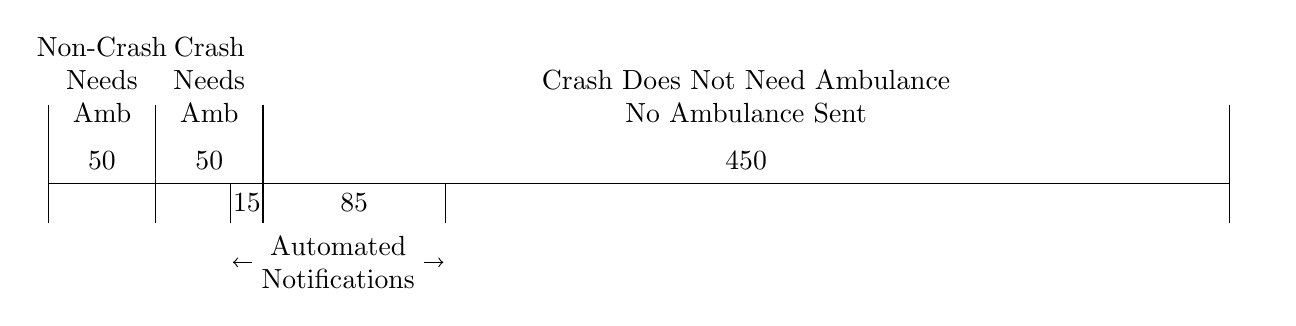
\begin{tikzpicture}[x=0.02727cm, y=0.5cm, font=\normalfont\normalsize]
	\path (568,0) circle (0pt); % Add 0.5 cm on right for margin
	\draw [color=black] (0,0) -- (550,0);
	\draw [color=black] (0,2) -- (0,-1);
	\draw [color=black] (50,2) -- (50,-1);
	\draw [color=black] (100,2) -- (100,-1);
	\draw [color=black] (550,2) -- (550,-1);
	\node (A) at (25,0) {};
	\node (B) [above=-2pt of A, align=center, text=black] {
		Non-Crash \\ Needs \\ Amb \\[0.5em] 50
	};
	\node (C) at (75,0) {};
	\node (D) [above=-2pt of C, align=center, text=black] {
		Crash \\ Needs \\ Amb \\[0.5em] 50
	};
	\node (E) at (325,0) {};
	\node (F) [above=-2pt of E, align=center, text=black] {
		Crash Does Not Need Ambulance \\ No Ambulance Sent \\[0.5em]  450
	};
	\draw [color=black] (85,0) -- (85,-1);
	\draw [color=black] (185,0) -- (185,-1);
	\path (85,0) -- (100,0) node [below, midway, color=black] {
		15
		};
	\path (100,0) -- (185,0) node [below, midway, color=black] {
		85
	};
	
	\draw [<->, color=black]  (86,-2) -- (184,-2) 
		node [midway, color=black, fill=white, align=center] 
		{Automated \\ Notifications};
%	
%	\path (85,-1) -- (185,-1) node 
%		[below, midway, color=black, align=center] {
%		Automated \\ Notifications
%	};
\end{tikzpicture}

\caption{\normalfont\normalsize Springfield before implementing immediate dispatch of ambulances.  Figure accompanies \S\ref{intro_scenario}}
\label{intro_springfield_before}
\end{figure}

\FloatBarrier

If Springfield were to implement an AI recommendation system to immediately dispatch ambulances based on automated calls from cell phones, the recommendations would not perfectly predict which crash persons need an ambulance.    See Figure \ref{intro_springfield_after}, where we have zoomed in on the left side of Figure \ref{intro_springfield_before}. In our per-100-ambulances-currently-sent proportions, the recommendation system would classify each of the automated notifications as needing or not needing an ambulance.  

Of the fifteen automated crash notifications that need an ambulance, the system would correctly classify some of them as needing an ambulance (True Positives, TP), and those crash persons would get medical attention more promptly, which is the goal and benefit of the recommendation system.  The rest of those fifteen would be incorrectly classified as probably not needing an ambulance with a recommendation to wait for a call from an eyewitness before sending one. (False Negatives, FN).  Note that the false negatives get an ambulance just as quickly under the new system as under the old,  with an ambulance dispatched upon call from an eyewitness.  

Of the 85 automated notifications that do need an ambulance, some would be correctly classified (True Negatives, TN), but some would be incorrectly classified and we would immediately dispatch an unneeded ambulance (False Positives, FP).  Besides administration, those additional ambulance runs are the cost of immediately dispatching ambulances.  In the short term those additional ambulance runs could be more than current resources (ambulances and their teams) could handle, and in the long term could be unnacceptably expensive.  

\begin{figure}[h]
	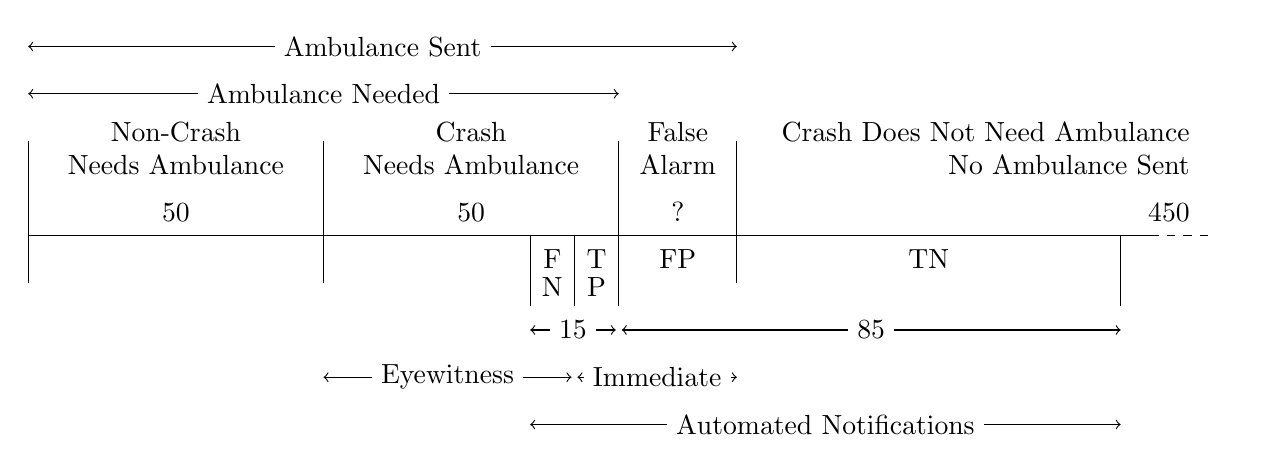
\begin{tikzpicture}[x=0.075cm, y=0.6cm, font=\normalfont\normalsize] % 15 cm wide
	\path (207,0) circle (0pt);
	\draw [color=black] (0,0) -- (190,0);
	\draw [color=black, dashed] (190,0) -- (200,0);
	\draw [color=black] (0,2) -- (0,-1);
	\draw [color=black] (50,2) -- (50,-1);
	\draw [color=black] (100,2) -- (100,-1.5);
	\draw [color=black] (120,2) -- (120,-1);
	\node (A) at (25,0) {};
	\node (B) [above=-2pt of A, align=center, text=black] {
		Non-Crash \\ Needs Ambulance \\[0.5em] 50
	};
	\node (C) at (75,0) {};
	\node (D) [above=-2pt of C, align=center, text=black] {
		Crash \\ Needs Ambulance \\[0.5em] 50
	};
	\node (E) at (200,0) {};
	\node (F) [above left =-2pt and 0pt of E, align=right, text=black] {
		Crash Does Not Need Ambulance \\ No Ambulance Sent \\[0.5em] 450
	};
	\node (G) at (110,0) {};
	\node (H) [above=-2pt of G, align=center, text=black] {
		False \\ Alarm \\[0.5em] ?
	};

	\draw [color=black] (85,0) -- (85,-1.5);
	\draw [color=black] (185,0) -- (185,-1.5);
%	\path (85,-2) -- (100,-2) node [below, midway, color=black] {15};
%	\path (100,-1) -- (185,-1) node [below, midway, color=black] {85};
	
	\draw [<->, color=black]  (100.5,-2) -- (185,-2) 
		node [midway, color=black, fill=white, align=center] 
		{85};

	\draw [<->, color=black]  (85,-2) -- (99.5,-2) 
		node [midway, color=black, fill=white, align=center] 
		{15};

	\draw [<->, color=black]  (50,-3) -- (92,-3) 
		node [midway, color=black, fill=white, align=center] 
		{Eyewitness};

	\draw [<->, color=black]  (93,-3) -- (120,-3) 
		node [midway, color=black, fill=white, align=center] 
		{Immediate};

	\draw [<->, color=black]  (85,-4) -- (185,-4) 
		node [midway, color=black, fill=white, align=center] 
		{Automated Notifications};

	\draw [<->, color=black]  (0,3) -- (100,3) 
		node [midway, color=black, fill=white, align=center] 
		{Ambulance Needed};

	\draw [<->, color=black]  (0,4) -- (120,4) 
		node [midway, color=black, fill=white, align=center] 
		{Ambulance Sent};

%	\node (G) at (110,2) [color=black, align=left] {False \\  Alarm};
	\path (100,-0.5) -- (120,-0.5) node [midway, color=black] {FP};
	\path (120,-0.5) -- (185,-0.5) node [midway, color=black] {TN};
	\draw [color=black] (92.5,0) -- (92.5,-1.5);
	\path (85,-0.5) -- (92.5,-0.5) node [midway, color=black] {F};
	\path (85,-1.2) -- (92.5,-1.0) node [midway, color=black] {N};
	\path (100,-0.5) -- (92.5,-0.5) node [midway, color=black] {T};
	\path (100,-1.2) -- (92.5,-1.0) node [midway, color=black] {P};
\end{tikzpicture}

\caption{\normalfont\normalsize Springfield after implementing immediate dispatch of ambulances.  Figure accompanies \S\ref{intro_scenario}}
\label{intro_springfield_after}
\end{figure}

\FloatBarrier

The leaders of Springfield need to find a balance between the benefit of more prompt medical attention and the cost of sending more ambulances.  The tradeoff of lives and money is not ethically or morally comfortable, but that is the choice governments make when they set budgets for health care and emergency services.  In the confusion matrices in Figure \ref{intro_confusion}, Springfield would love to increase TP without increasing FP, but the recommendation system will not give perfect predictions.  

\begin{figure}[h]
\begin{minipage}{\linewidth}
{\normalfont\normalsize
\begin{tabular}{p{2in}p{3in}}
\begin{tabular}{c c  | c | c | c}
	& \multicolumn{1}{c}{} & \multicolumn{2}{c}{Prediction}  \cr
	&\multicolumn{1}{c}{} & \multicolumn{1}{c}{PN} & \multicolumn{1}{c}{PP} \cr\cline{3-4}
	\multirow{2}{*}{Actual} & N & TN & FP \vrule width 0pt height 10pt depth 2pt \cr\cline{3-4}
	 & P & FN & TP	\vrule width 0pt height 10pt depth 4pt \cr\cline{3-4}
\end{tabular}
&
\begin{tabular}{c c  | c | c | c}
	\multicolumn{2}{@{}l}{Recommendation} & \multicolumn{1}{ @{} c @{} }{Wait for Call} & \multicolumn{1}{ @{} c @{} }{Immediately}   \cr
	&\multicolumn{1}{ @{} c @{} }{} & \multicolumn{1}{ @{} c @{} }{from Eyewitness} & \multicolumn{1}{ @{} c @{} }{Dispatch} \cr\cline{3-4}
	Needs & No & Correct & Increased Cost
		\vrule width 0pt height 10pt depth 2pt \cr\cline{3-4}
	Ambulance? \ \ &Yes & 
		Normal Delay & \ Prompt Medical Help \
		\vrule width 0pt height 10pt depth 4pt \cr\cline{3-4}
\end{tabular}
\cr		
\end{tabular}
}
\end{minipage}
\caption{\normalfont\normalsize Confusion matrix for ambulance dispatch.  Figure accompanies \S\ref{intro_scenario}}
\label{intro_confusion}
\end{figure}

\FloatBarrier

Building Springfield's AI recommendation system starts with an historical dataset with the features the emergency dispatchers will have at the time of the automated notification, like time of day, weather, maybe age and sex, and possibly more information, and whether that historical crash person needed an ambulance (supervised learning).  A machine learning algorithm learns a model of the data, and when an automated crash notification comes in, given the data available, the model returns a value $p \in [0,1]$ that increases with the probability that the crash person needs an ambulance.  Choosing $p=1$ would mean never immediately dispatching an ambulance, and $p=0$ would be always.  The city council and mayor need to choose a decision threshold $\theta$ such that if, for a particular crash notification, $p>\theta$, then immediately dispatch an ambulance; if $p<\theta$, wait for a call from an eyewitness.  

The histogram in Figure \ref{intro_ideal} shows typical model output.  The model generally gives lower $p$ values to crash persons who do not need an ambulance (Neg) and higher $p$ values to crash persons who do need an ambulance (Pos), but there is significant overlap.  The most obvious feature of the histogram is the class imbalance, that there are many more Neg than Pos, in fact $85/15 \approx 6$ Neg for each Pos.  

  Given a choice of $\theta$, Springfield would immediately dispatch ambulances to all of the crashes to the right of $\theta$.  The Pos (Needs ambulance) to the right of $\theta$ (TP) would get more prompt medical attention, but the Neg (Does not need ambulance) to the right (FP) would be wasted ambulance runs.  At $\theta = 0.8$, TP and FP are about equal, but as we consider smaller $\theta$ the number of TP increases by smaller and smaller amounts while the number of FP grows dramatically.  

\begin{figure}[h]
\centering
	\input{../Keras/Images/Ideal_Pred_Wide.pgf}	
\caption{\normalfont\normalsize Example model test results.  Figure accompanies \S\ref{intro_scenario}}
\label{intro_ideal}
\end{figure}

\FloatBarrier

We will consider three ways the leaders of Springfield can think about how to choose $\theta$, three metrics for political decision thresholds, detailed in \S \ref{political_decisions}.

\begin{enumerate}
	\item Percent increase in number of ambulance calls
	\item Percent of immediately dispatched ambulances that are actually needed
	\item Minimum probability that an immediately dispatched ambulance is actually needed
\end{enumerate}









%%%%% Methods
\section{Methods}\label{sec:Methods}
\input{Methods}
%\section{Methods\_Old}
%\input{Methods_Old}
%\section{Methods\_for\_TRpC}
%%%%%% Methods_for_TRpC

\subsection{Goal}

The goal of this paper is to show one method for determining, for different levels of available data and criteria reflecting different political choices, how well a machine learning model can predict whether an emergency call center should automatically dispatch an ambulance based on an automated crash notification.  

Usually a crash notification comes to an emergency dispatcher from an eyewitness who can say whether there are injuries requiring medical attention.  With an automated crash notification, however, that information is not available.  We want to know whether, or to what degree, we can infer from information that is available whether it is likely that the phone's user needs an ambulance, and thus whether we should automatically dispatch an ambulance to the scene.  

We will use an existing dataset to build models that give us the probability.  For each of several different political realities and goals, we will choose the most useful model and find a threshold above which the emergency call center should automatically dispatch an ambulance.  We will consider three different levels of available information, with ``Easy'' using information already available, ``Medium'' adding information that requires a higher level of planning and preparation, and ``Hard'' requiring cooperation between public and private data sources with possible conflicts of privacy and confidentiality.  

From the results, a local government would have information on which to base a decision about whether to implement an automated dispatch system and what level of data to provide.  The ultimate decision is political, weighing lives against money.

\subsection{Dataset}

Ideally, we would use a dataset of crashes with an automated notification, but we have not found such a dataset that is publicly available.  Working with such a private dataset would be an important avenue of future research.

We will use the Crash Report Sampling System (CRSS) from 2016 to 2021.  The CRSS is a curated sample of crashes in the US, weighted to more serious crashes such that 17\% of the crash persons needed an ambulance, significantly more than the proportion of all reported crashes needing an ambulance, between 2 and 3 percent.  Since most low-speed crashes would have a crash profile similar to hard braking, they would not spawn an automated notification, so it is reasonable to assume that the set of crashes with automated notifications would have a higher percentage of persons needing an ambulance.  

We will use the CRSS as a proxy for the set of crashes with automatic crash notifications, acknowledging that we do not know how good of a proxy it is.  The primary merit of CRSS for our work is that it is publicly available so that our work can be critiqued, adapted, and expanded by others.  

We merged the \verb|accident.csv|, \verb|vehicle.csv|, and \verb|person.csv| files in the six years.  We dropped many features that were irrelevant, most because they were unique to each vehicle like a VIN (Vehicle Identification Number), with no predictive power, just random noise.  We also dropped the 33,776 persons in crashes involving a pedestrian, because the deceleration profile of hitting a pedestrian or bicycle would not be different enough from hard braking to trigger an automated crash notification.  

After removing repeated and irrelevant features and pedestrian crashes, we have 118 features describing 713,566 crash persons.  Later we removed more that have more than 20\% of the values missing or only have data for some years, and features with imputed missing values to get 78 features.

For full details, see the \verb|Ambulance_Dispatch_01_Get_Data.ipynb| file.  

\subsection{Binning Categories}

All of the CRSS data is discrete, but some features are ordered, like \verb|HOUR| and \verb|AGE|, and others are unordered, like \verb|MAKE_MOD|.  Reducing the dimensionality of the machine learning modeling by binning the categories into less than ten per feature is ideal.  

Some features like \verb|HOUR| we binned by hand.  We looked at the proportion of crash persons hospitalized at each hour and found clear places to break it into seven contiguous but not equal blocks.  When we looked at \verb|AGE|, we considered breaking it into decades, but found that ages 15-18 have a far lower hospitalization rate than those a little younger or older, and there was a shift at about age 53 and again around age 74, so we binned it accordingly.  

Some features like \verb|MAKE_MOD|m which has 1,210 unique values, we binned by imposing an order, ordering by the proportion of crash persons hospitalized, then cutting the ordered list into five new categories plus ``Unknown.''  



For full details, see 
\verb|Ambulance_Dispatch_02_Correlation.ipynb| and 
\verb|Ambulance_Dispatch_03_Bin_Data.ipynb|.

\subsection{Imputing Missing Data}

For reasons of historical consistency going back to 1982 with the predecessors of CRSS, CRSS imputes missing values for some features but not others, using IVEware, Imputation and Variation Estimation Software from the Institute for Social Research at the University of Michigan.  Fortunately, when CRSS gives a feature with imputed values, it also retains the feature with values signifying ``Unknown.'' CRSS has a very helpful report on its imputation methods.  We have not seen in the literature where someone has used IVEware to impute the other features and compared it to other methods.  

At this point we have 78 unimputed features, and only 250,389 out of 713,566 samples (35\%) did not have missing values in those 78 features.  We compared three methods for imputing missing values.  

\begin{itemize}
	\item IVEware
	\item Imputation to Mode
	\item Round-Robin Random Forest using Imputation to Mode as the starting point
\end{itemize}

We found that the Random Forest method was best.  

For full details and analysis, see 
\verb|Ambulance_Dispatch_04_Impute_Missing_Data.ipynb|.

\subsection{Order of Operations}

We also considered whether the order of operations made a difference, whether we should bin first, then impute, or impute using the raw data, then bin.  We tried both methods over several runs and found that the difference between methods was about the same as the difference between runs of the same method with different random seeds.  Since IVEware can only handle up to about forty categories in each categorical field, we had had to bin some fields first either way, so we chose to bin first, then impute.  

For full details and analysis, see 
\verb|Ambulance_Dispatch_05_IVEware_Order_of_Operations.ipynb|.















%%%%% Results
\section{Results}\label{sec:Results}

%%%%% Conclusions
\section{Conclusions}\label{Conclusions}

%%%%%
\section{Discussion}\label{Discussion}
%\input{Discussion}

%%%%% Future Work
\section{Future Work}\label{FutureWork}
%\input{Future_Work}


%%%%%
\section*{Funding Statement}

This research did not receive any specific grant from funding agencies in the public, commercial, or not-for-profit sectors.

%%%%% Conflict of Interest
\section*{Conflict of Interest}

Declarations of interest: none
%The authors have no relevant financial or non-financial interests to disclose.

%%%%% Acknowledgements
\section*{Acknowledgements}

George Broussard 
%[STUDENT]
contributed to this work in the 
%[FUNDED PROGRAM]
NSF Research Experiences for Undergraduates program.

%%%%% Data Availability
\section*{Data Availability}

The CRSS data is publicly available at 

\url{https://www.nhtsa.gov/crash-data-systems/crash-report-sampling-system}

All of the code and generated data, tables, and graphs are available at 
\url{http://www.github.com/bburkman}

%%%%% Declaration of Generative AI and AI-assisted technologies in the writing process
%\section*{Declaration of Generative AI and AI-assisted technologies in the writing process}



\begin{comment}
% Figure
\begin{figure}[<options>]
	\centering
		\includegraphics[<options>]{}
	  \caption{}\label{fig1}
\end{figure}


\begin{table}[<options>]
\caption{}\label{tbl1}
\begin{tabular*}{\tblwidth}{@{}LL@{}}
\toprule
  &  \\ % Table header row
\midrule
 & \\
 & \\
 & \\
 & \\
\bottomrule
\end{tabular*}
\end{table}
\end{comment}

% Uncomment and use as the case may be
%\begin{theorem} 
%\end{theorem}

% Uncomment and use as the case may be
%\begin{lemma} 
%\end{lemma}

%% The Appendices part is started with the command \appendix;
%% appendix sections are then done as normal sections
%% \appendix

%\section{}\label{}

% To print the credit authorship contribution details
\printcredits

%% Loading bibliography style file
%\bibliographystyle{model1-num-names}
\bibliographystyle{cas-model2-names}

% Loading bibliography database
\bibliography{Paper_Summer_2022.bib}

\begin{comment}
% Biography
\bio{}
% Here goes the biography details.
\endbio

\bio{pic1}
% Here goes the biography details.
\endbio
\end{comment}

\end{document}

